\documentclass[dvisvgm]{standalone}
\begin{document}
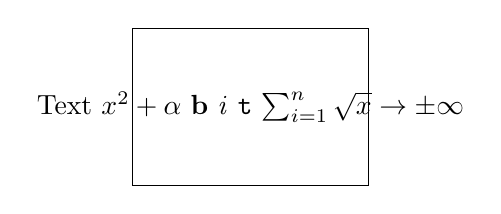
\begin{tikzpicture}
  \draw (0,0) rectangle (3,2);
  \node at (1.5,1) {Text $x^2+\alpha$ \textbf{b} \textit{i} \texttt{t} $\sum_{i=1}^{n}\sqrt{x}\to\pm\infty$};
\end{tikzpicture}
\begin{circuitikz}
  \draw (0,0) to[V, l=$V_s$] (0,3) to[R, l=$R_1$] (3,3) to[R, l=$R_2$] (3,0) -- (0,0);
\end{circuitikz}
\end{document}
